% Options for packages loaded elsewhere
\PassOptionsToPackage{unicode}{hyperref}
\PassOptionsToPackage{hyphens}{url}
\PassOptionsToPackage{dvipsnames,svgnames,x11names}{xcolor}
%
\documentclass[
  letterpaper,
  DIV=11,
  numbers=noendperiod]{scrartcl}

\usepackage{amsmath,amssymb}
\usepackage{iftex}
\ifPDFTeX
  \usepackage[T1]{fontenc}
  \usepackage[utf8]{inputenc}
  \usepackage{textcomp} % provide euro and other symbols
\else % if luatex or xetex
  \usepackage{unicode-math}
  \defaultfontfeatures{Scale=MatchLowercase}
  \defaultfontfeatures[\rmfamily]{Ligatures=TeX,Scale=1}
\fi
\usepackage{lmodern}
\ifPDFTeX\else  
    % xetex/luatex font selection
\fi
% Use upquote if available, for straight quotes in verbatim environments
\IfFileExists{upquote.sty}{\usepackage{upquote}}{}
\IfFileExists{microtype.sty}{% use microtype if available
  \usepackage[]{microtype}
  \UseMicrotypeSet[protrusion]{basicmath} % disable protrusion for tt fonts
}{}
\makeatletter
\@ifundefined{KOMAClassName}{% if non-KOMA class
  \IfFileExists{parskip.sty}{%
    \usepackage{parskip}
  }{% else
    \setlength{\parindent}{0pt}
    \setlength{\parskip}{6pt plus 2pt minus 1pt}}
}{% if KOMA class
  \KOMAoptions{parskip=half}}
\makeatother
\usepackage{xcolor}
\setlength{\emergencystretch}{3em} % prevent overfull lines
\setcounter{secnumdepth}{-\maxdimen} % remove section numbering
% Make \paragraph and \subparagraph free-standing
\makeatletter
\ifx\paragraph\undefined\else
  \let\oldparagraph\paragraph
  \renewcommand{\paragraph}{
    \@ifstar
      \xxxParagraphStar
      \xxxParagraphNoStar
  }
  \newcommand{\xxxParagraphStar}[1]{\oldparagraph*{#1}\mbox{}}
  \newcommand{\xxxParagraphNoStar}[1]{\oldparagraph{#1}\mbox{}}
\fi
\ifx\subparagraph\undefined\else
  \let\oldsubparagraph\subparagraph
  \renewcommand{\subparagraph}{
    \@ifstar
      \xxxSubParagraphStar
      \xxxSubParagraphNoStar
  }
  \newcommand{\xxxSubParagraphStar}[1]{\oldsubparagraph*{#1}\mbox{}}
  \newcommand{\xxxSubParagraphNoStar}[1]{\oldsubparagraph{#1}\mbox{}}
\fi
\makeatother

\usepackage{color}
\usepackage{fancyvrb}
\newcommand{\VerbBar}{|}
\newcommand{\VERB}{\Verb[commandchars=\\\{\}]}
\DefineVerbatimEnvironment{Highlighting}{Verbatim}{commandchars=\\\{\}}
% Add ',fontsize=\small' for more characters per line
\usepackage{framed}
\definecolor{shadecolor}{RGB}{241,243,245}
\newenvironment{Shaded}{\begin{snugshade}}{\end{snugshade}}
\newcommand{\AlertTok}[1]{\textcolor[rgb]{0.68,0.00,0.00}{#1}}
\newcommand{\AnnotationTok}[1]{\textcolor[rgb]{0.37,0.37,0.37}{#1}}
\newcommand{\AttributeTok}[1]{\textcolor[rgb]{0.40,0.45,0.13}{#1}}
\newcommand{\BaseNTok}[1]{\textcolor[rgb]{0.68,0.00,0.00}{#1}}
\newcommand{\BuiltInTok}[1]{\textcolor[rgb]{0.00,0.23,0.31}{#1}}
\newcommand{\CharTok}[1]{\textcolor[rgb]{0.13,0.47,0.30}{#1}}
\newcommand{\CommentTok}[1]{\textcolor[rgb]{0.37,0.37,0.37}{#1}}
\newcommand{\CommentVarTok}[1]{\textcolor[rgb]{0.37,0.37,0.37}{\textit{#1}}}
\newcommand{\ConstantTok}[1]{\textcolor[rgb]{0.56,0.35,0.01}{#1}}
\newcommand{\ControlFlowTok}[1]{\textcolor[rgb]{0.00,0.23,0.31}{\textbf{#1}}}
\newcommand{\DataTypeTok}[1]{\textcolor[rgb]{0.68,0.00,0.00}{#1}}
\newcommand{\DecValTok}[1]{\textcolor[rgb]{0.68,0.00,0.00}{#1}}
\newcommand{\DocumentationTok}[1]{\textcolor[rgb]{0.37,0.37,0.37}{\textit{#1}}}
\newcommand{\ErrorTok}[1]{\textcolor[rgb]{0.68,0.00,0.00}{#1}}
\newcommand{\ExtensionTok}[1]{\textcolor[rgb]{0.00,0.23,0.31}{#1}}
\newcommand{\FloatTok}[1]{\textcolor[rgb]{0.68,0.00,0.00}{#1}}
\newcommand{\FunctionTok}[1]{\textcolor[rgb]{0.28,0.35,0.67}{#1}}
\newcommand{\ImportTok}[1]{\textcolor[rgb]{0.00,0.46,0.62}{#1}}
\newcommand{\InformationTok}[1]{\textcolor[rgb]{0.37,0.37,0.37}{#1}}
\newcommand{\KeywordTok}[1]{\textcolor[rgb]{0.00,0.23,0.31}{\textbf{#1}}}
\newcommand{\NormalTok}[1]{\textcolor[rgb]{0.00,0.23,0.31}{#1}}
\newcommand{\OperatorTok}[1]{\textcolor[rgb]{0.37,0.37,0.37}{#1}}
\newcommand{\OtherTok}[1]{\textcolor[rgb]{0.00,0.23,0.31}{#1}}
\newcommand{\PreprocessorTok}[1]{\textcolor[rgb]{0.68,0.00,0.00}{#1}}
\newcommand{\RegionMarkerTok}[1]{\textcolor[rgb]{0.00,0.23,0.31}{#1}}
\newcommand{\SpecialCharTok}[1]{\textcolor[rgb]{0.37,0.37,0.37}{#1}}
\newcommand{\SpecialStringTok}[1]{\textcolor[rgb]{0.13,0.47,0.30}{#1}}
\newcommand{\StringTok}[1]{\textcolor[rgb]{0.13,0.47,0.30}{#1}}
\newcommand{\VariableTok}[1]{\textcolor[rgb]{0.07,0.07,0.07}{#1}}
\newcommand{\VerbatimStringTok}[1]{\textcolor[rgb]{0.13,0.47,0.30}{#1}}
\newcommand{\WarningTok}[1]{\textcolor[rgb]{0.37,0.37,0.37}{\textit{#1}}}

\providecommand{\tightlist}{%
  \setlength{\itemsep}{0pt}\setlength{\parskip}{0pt}}\usepackage{longtable,booktabs,array}
\usepackage{calc} % for calculating minipage widths
% Correct order of tables after \paragraph or \subparagraph
\usepackage{etoolbox}
\makeatletter
\patchcmd\longtable{\par}{\if@noskipsec\mbox{}\fi\par}{}{}
\makeatother
% Allow footnotes in longtable head/foot
\IfFileExists{footnotehyper.sty}{\usepackage{footnotehyper}}{\usepackage{footnote}}
\makesavenoteenv{longtable}
\usepackage{graphicx}
\makeatletter
\newsavebox\pandoc@box
\newcommand*\pandocbounded[1]{% scales image to fit in text height/width
  \sbox\pandoc@box{#1}%
  \Gscale@div\@tempa{\textheight}{\dimexpr\ht\pandoc@box+\dp\pandoc@box\relax}%
  \Gscale@div\@tempb{\linewidth}{\wd\pandoc@box}%
  \ifdim\@tempb\p@<\@tempa\p@\let\@tempa\@tempb\fi% select the smaller of both
  \ifdim\@tempa\p@<\p@\scalebox{\@tempa}{\usebox\pandoc@box}%
  \else\usebox{\pandoc@box}%
  \fi%
}
% Set default figure placement to htbp
\def\fps@figure{htbp}
\makeatother

\KOMAoption{captions}{tableheading}
\makeatletter
\@ifpackageloaded{caption}{}{\usepackage{caption}}
\AtBeginDocument{%
\ifdefined\contentsname
  \renewcommand*\contentsname{Table of contents}
\else
  \newcommand\contentsname{Table of contents}
\fi
\ifdefined\listfigurename
  \renewcommand*\listfigurename{List of Figures}
\else
  \newcommand\listfigurename{List of Figures}
\fi
\ifdefined\listtablename
  \renewcommand*\listtablename{List of Tables}
\else
  \newcommand\listtablename{List of Tables}
\fi
\ifdefined\figurename
  \renewcommand*\figurename{Figure}
\else
  \newcommand\figurename{Figure}
\fi
\ifdefined\tablename
  \renewcommand*\tablename{Table}
\else
  \newcommand\tablename{Table}
\fi
}
\@ifpackageloaded{float}{}{\usepackage{float}}
\floatstyle{ruled}
\@ifundefined{c@chapter}{\newfloat{codelisting}{h}{lop}}{\newfloat{codelisting}{h}{lop}[chapter]}
\floatname{codelisting}{Listing}
\newcommand*\listoflistings{\listof{codelisting}{List of Listings}}
\makeatother
\makeatletter
\makeatother
\makeatletter
\@ifpackageloaded{caption}{}{\usepackage{caption}}
\@ifpackageloaded{subcaption}{}{\usepackage{subcaption}}
\makeatother

\usepackage{bookmark}

\IfFileExists{xurl.sty}{\usepackage{xurl}}{} % add URL line breaks if available
\urlstyle{same} % disable monospaced font for URLs
\hypersetup{
  pdftitle={Introduction to Python},
  pdfauthor={Verjinia Metodieva and Daniel Parthier},
  colorlinks=true,
  linkcolor={blue},
  filecolor={Maroon},
  citecolor={Blue},
  urlcolor={Blue},
  pdfcreator={LaTeX via pandoc}}


\title{Introduction to Python}
\author{Verjinia Metodieva and Daniel Parthier}
\date{2025-01-21}

\begin{document}
\maketitle


\section{Why would you code?}\label{why-would-you-code}

Motivation

\begin{itemize}
\tightlist
\item
  Saving time
\item
  Reproducible workflow
\item
  Flexibility
\item
  Unlimited creativity
\end{itemize}

\section{Goal of today}\label{goal-of-today}

\begin{Shaded}
\begin{Highlighting}[]
\CommentTok{\# This script exports metadata information to a JSON file.}
\CommentTok{\# The metadata includes the author, date, and length of the data.}
\CommentTok{\# The output is saved to \textquotesingle{}data/data\_info.json\textquotesingle{}.}
\ImportTok{import}\NormalTok{ json}
\NormalTok{cell\_count }\OperatorTok{=}\NormalTok{ [}\DecValTok{1}\NormalTok{,}\DecValTok{1}\NormalTok{,}\DecValTok{4}\NormalTok{,}\DecValTok{5}\NormalTok{,}\DecValTok{2}\NormalTok{]}
\NormalTok{cell\_count.sort()}
\NormalTok{list\_length }\OperatorTok{=} \BuiltInTok{len}\NormalTok{(cell\_count)}
\NormalTok{output\_file }\OperatorTok{=} \StringTok{\textquotesingle{}data/data\_info.json\textquotesingle{}}
\NormalTok{output\_data }\OperatorTok{=}\NormalTok{ \{}
    \StringTok{\textquotesingle{}author\textquotesingle{}}\NormalTok{: }\StringTok{\textquotesingle{}Doe, John\textquotesingle{}}\NormalTok{,}
    \StringTok{\textquotesingle{}date\textquotesingle{}}\NormalTok{: }\StringTok{\textquotesingle{}2025{-}01{-}10\textquotesingle{}}\NormalTok{,}
    \StringTok{\textquotesingle{}length\textquotesingle{}}\NormalTok{: list\_length}
\NormalTok{\}}
\ControlFlowTok{with} \BuiltInTok{open}\NormalTok{(output\_file, }\StringTok{\textquotesingle{}w\textquotesingle{}}\NormalTok{) }\ImportTok{as}\NormalTok{ f:}
\NormalTok{    json.dump(output\_data, f)}
\end{Highlighting}
\end{Shaded}

This is an example to showcase what we will achieve today.

\section{Basic usage}\label{basic-usage}

\begin{itemize}
\tightlist
\item
  Can be run from the terminal/console as well

  \begin{itemize}
  \tightlist
  \item
    Start python by typing \texttt{python}/\texttt{python3} into the
    console
  \item
    You can quit by typing \texttt{quit()} into the console
  \end{itemize}
\item
  Most of the time with a GUI (graphical user interface)
\item
  Sometimes code is run in document style (\emph{Jupyter Notebook})
\item
  Run scripts
\end{itemize}

The console is mainly used for quick testing of commands you will use
once and won't need to track. If you want to save your workflow or keep
track of what you did, a script is required. In principle, a script is
nothing else than a text file with a language-specific extension (.py).
The code is saved in such a file and can be used by activating the
script as a whole or running single code lines.

\subsection{Visual Studio Code}\label{visual-studio-code}

\begin{itemize}
\tightlist
\item
  1 of multiple options
  (\href{https://www.jetbrains.com/pycharm/}{PyCharm},
  \href{https://www.spyder-ide.org/}{Spyder})
\item
  VS Code offers multifunctionality and integration of useful extensions
  (Git, Remote Explorer, Jupyter, GitHub Copilot)
\end{itemize}

\pandocbounded{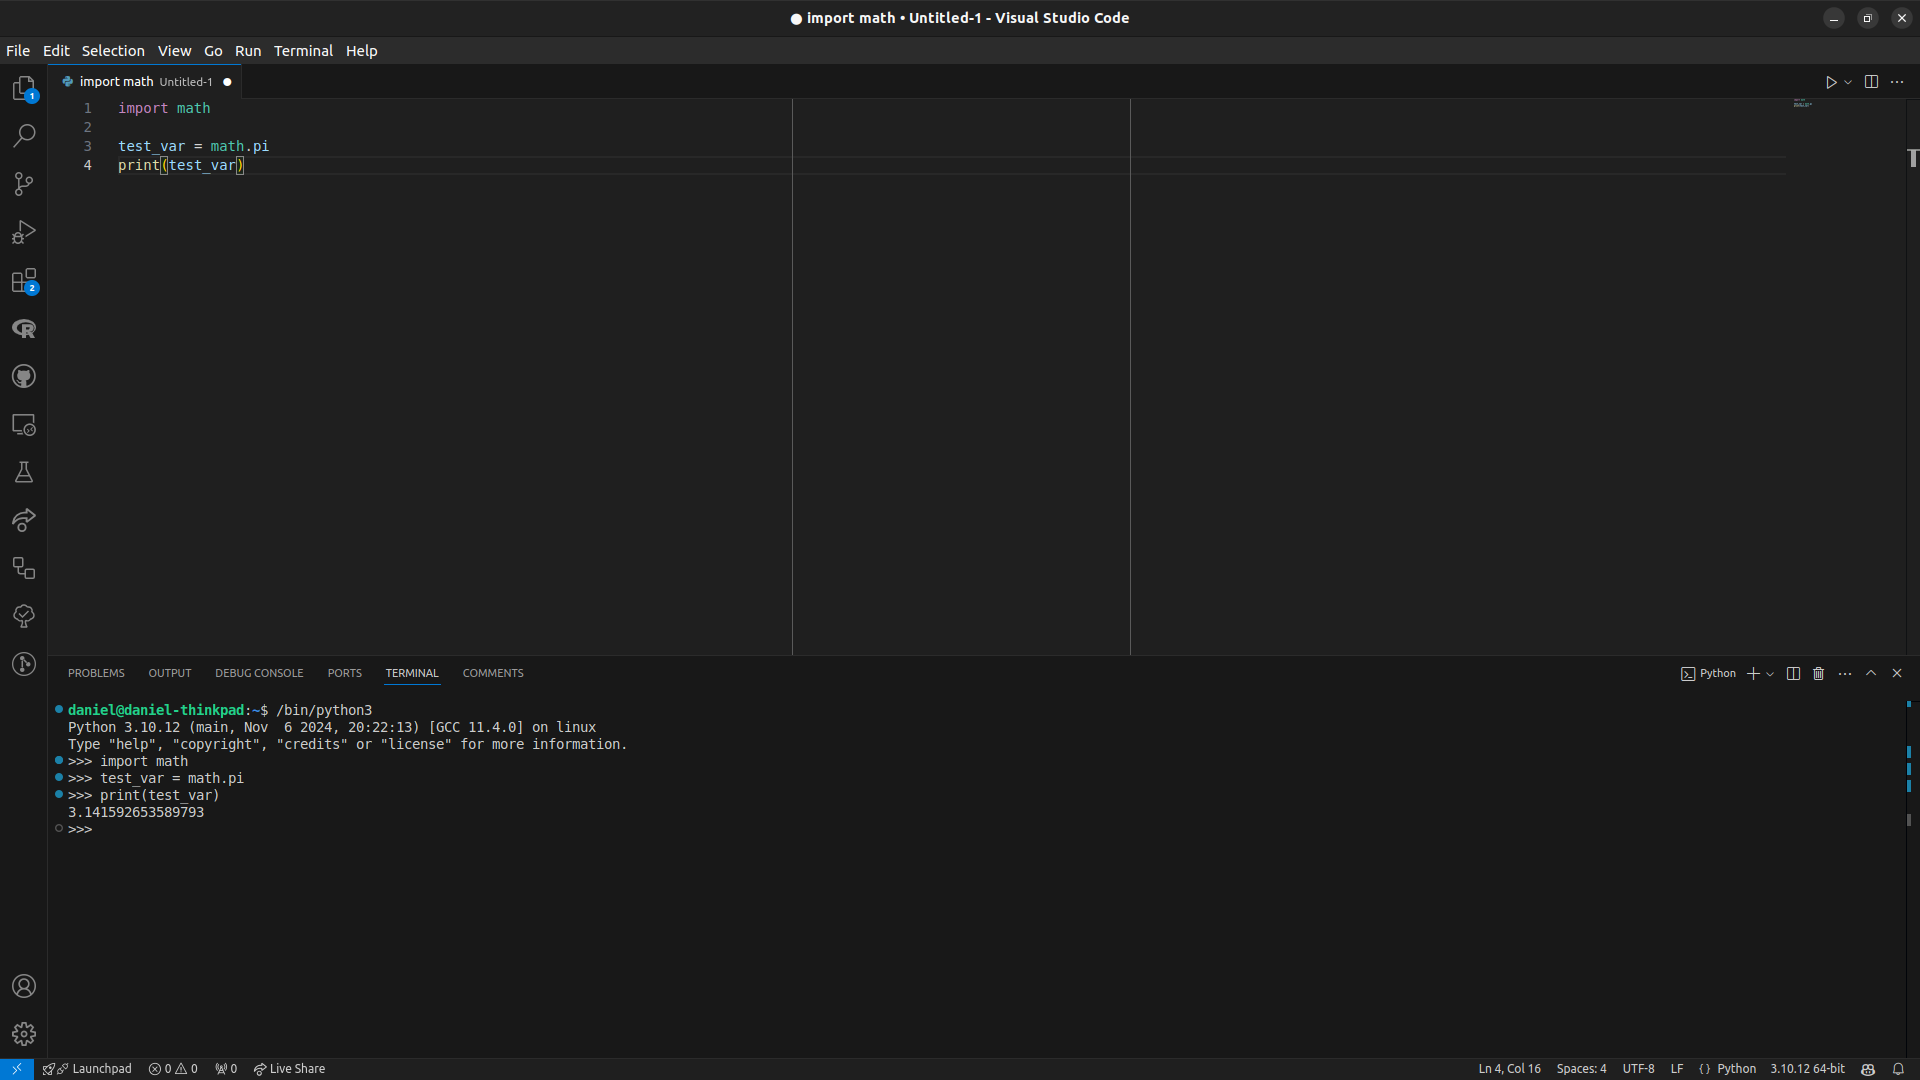
\includegraphics[keepaspectratio]{img/VSCode_script.png}}

A graphical user interface, like VS Code, provides code highlighting,
formatting, and completion. At the same time, it gives a structured
overview of a project. In the case of VS Code, you can use multiple
languages by just adding the appropriate extension.

\subsection{Visual Studio Code
(Features)}\label{visual-studio-code-features}

\begin{itemize}
\tightlist
\item
  Multi-language support (\emph{Python}, \emph{R}, \emph{Matlab},
  \emph{Julia}, \emph{C++}, etc.)
\item
  Set up your project (make environment, create files and folders)
\item
  Provide visual notation (code highlighting)
\item
  Auto-complete code snippets
\item
  Show documentation of functions
\item
  Find and fix errors in code (debugging)
\item
  Synchronise code with GitHub
\item
  And much more\ldots{}
\end{itemize}

\section{Environments}\label{environments}

\includegraphics[width=2.08333in,height=\textheight,keepaspectratio]{course_day_1_files/mediabag/organized-tool-drawe.jpg}
Photo by Stockcake

\begin{itemize}
\tightlist
\item
  Only bring the tools you need

  \begin{itemize}
  \tightlist
  \item
    Less bloated
  \item
    Fewer conflicts
  \end{itemize}
\item
  Only project-specific packages
\end{itemize}

\subsection{Make environment}\label{make-environment}

\begin{itemize}
\tightlist
\item
  Setting up an empty environment (get a drawer)
\item
  Can be done via terminal
\end{itemize}

\begin{Shaded}
\begin{Highlighting}[]
\ExtensionTok{python} \AttributeTok{{-}m}\NormalTok{ venv .venv}
\end{Highlighting}
\end{Shaded}

\begin{itemize}
\tightlist
\item
  Make one in VS Code

  \begin{itemize}
  \tightlist
  \item
    \texttt{CTRL\ +\ SHIFT\ +\ P} → type: \emph{env}
  \item
    Select: \emph{Create Environment}
  \end{itemize}
\end{itemize}

\subsection{Start environment}\label{start-environment}

\textbf{Windows}

\begin{Shaded}
\begin{Highlighting}[]
\ExtensionTok{.venv\textbackslash{}Scripts\textbackslash{}activate}
\end{Highlighting}
\end{Shaded}

\textbf{Unix/macOS}

\begin{Shaded}
\begin{Highlighting}[]
\BuiltInTok{source}\NormalTok{ .venv/bin/activate}
\end{Highlighting}
\end{Shaded}

\begin{itemize}
\tightlist
\item
  VS Code will start the environment for you
\end{itemize}

\subsection{Quit environment}\label{quit-environment}

\begin{Shaded}
\begin{Highlighting}[]
\ExtensionTok{deactivate}
\end{Highlighting}
\end{Shaded}

\section{Install packages}\label{install-packages}

\begin{itemize}
\tightlist
\item
  Package managers

  \begin{itemize}
  \item
    \emph{What are they?}
  \item
    pip (recommendeed)
  \item
    conda-forge (if you really have to)
  \end{itemize}
\end{itemize}

a collection of tools that automates the process of installing,
upgrading, configuring, and removing computer programs helps the user to
easily and consistently work with packages - installing, updating, etc.

\includegraphics[width=2.08333in,height=\textheight,keepaspectratio]{course_day_1_files/mediabag/TS-Inline-Image-2-20.png}

Trying my first note

\section{Import}\label{import}

When do you have to import?

\begin{itemize}
\tightlist
\item
  Only some functions are available by default
\end{itemize}

Let's open the `math' drawer!

\begin{Shaded}
\begin{Highlighting}[]
\ImportTok{import}\NormalTok{ math}
\end{Highlighting}
\end{Shaded}

This will open our math \emph{toolbox} drawer

\begin{itemize}
\tightlist
\item
  Pull out a tool to use it with the dot notation: {toolbox}{.}{tool}
\end{itemize}

\begin{Shaded}
\begin{Highlighting}[]
\NormalTok{math.pi}
\end{Highlighting}
\end{Shaded}

\begin{verbatim}
3.141592653589793
\end{verbatim}

\begin{Shaded}
\begin{Highlighting}[]
\NormalTok{math.sin(}\DecValTok{1}\NormalTok{)}
\end{Highlighting}
\end{Shaded}

\begin{verbatim}
0.8414709848078965
\end{verbatim}

Importing a package only has to happen once. By using
\texttt{import\ package} everything from the package will be made
available.

\subsection{Packages}\label{packages}

\subsection{Modules}\label{modules}

\section{Programming building blocks}\label{programming-building-blocks}

\subsection{Variables}\label{variables}

\subsection{(data-) types}\label{data--types}

\subsection{Simple functions}\label{simple-functions}

\subsection{Methods}\label{methods}

\section{Documentation}\label{documentation}

\section{Homework}\label{homework}




\end{document}
